\newpage
\section{Aufbau}
\begin{figure}
\begin{minipage}{0.49\textwidth}
Maßgebend für den Aufbau ist der $50 \si{\liter}$ große, mit Edelstahl umhüllte Szintillator vom Typ \enquote{NE 102} und mit Tuluol gefüllt. Diesem ist ein eigener Abschnitt gewidmet und dort entsprechend erläutert. \ref{kommt}
Mit ihm werden die einfallenden Myonen für die Detektion sichtbar gemacht. Da die entstehenden Signale schwach sind, bietet es sich an diese durch einen Sekundärelektronenverstärker, kurz SEV zu verstärken. An diesen Verstärkern ist für
die Funnktionalität eine Hochspannung angelegt. Dieser Teil des Aufbaus ist symetrisch an beiden Stirnseiten des Szintillator angebracht. So ist es also möglich die einfallenden Teilchen als Lichtsignal durch die SEV auszulesen.
Das Signal der zwei Sekundärelektronenverstärker kann durch vielerlei Gründe einseitig verschoben sein, das heißt es tritt durch asymetrische Verzögerungen eine zeitliche Differenz $\increment t$ auf.
\end{minipage}%
\begin{minipage}[h]{0.49\textwidth}
    \centering
    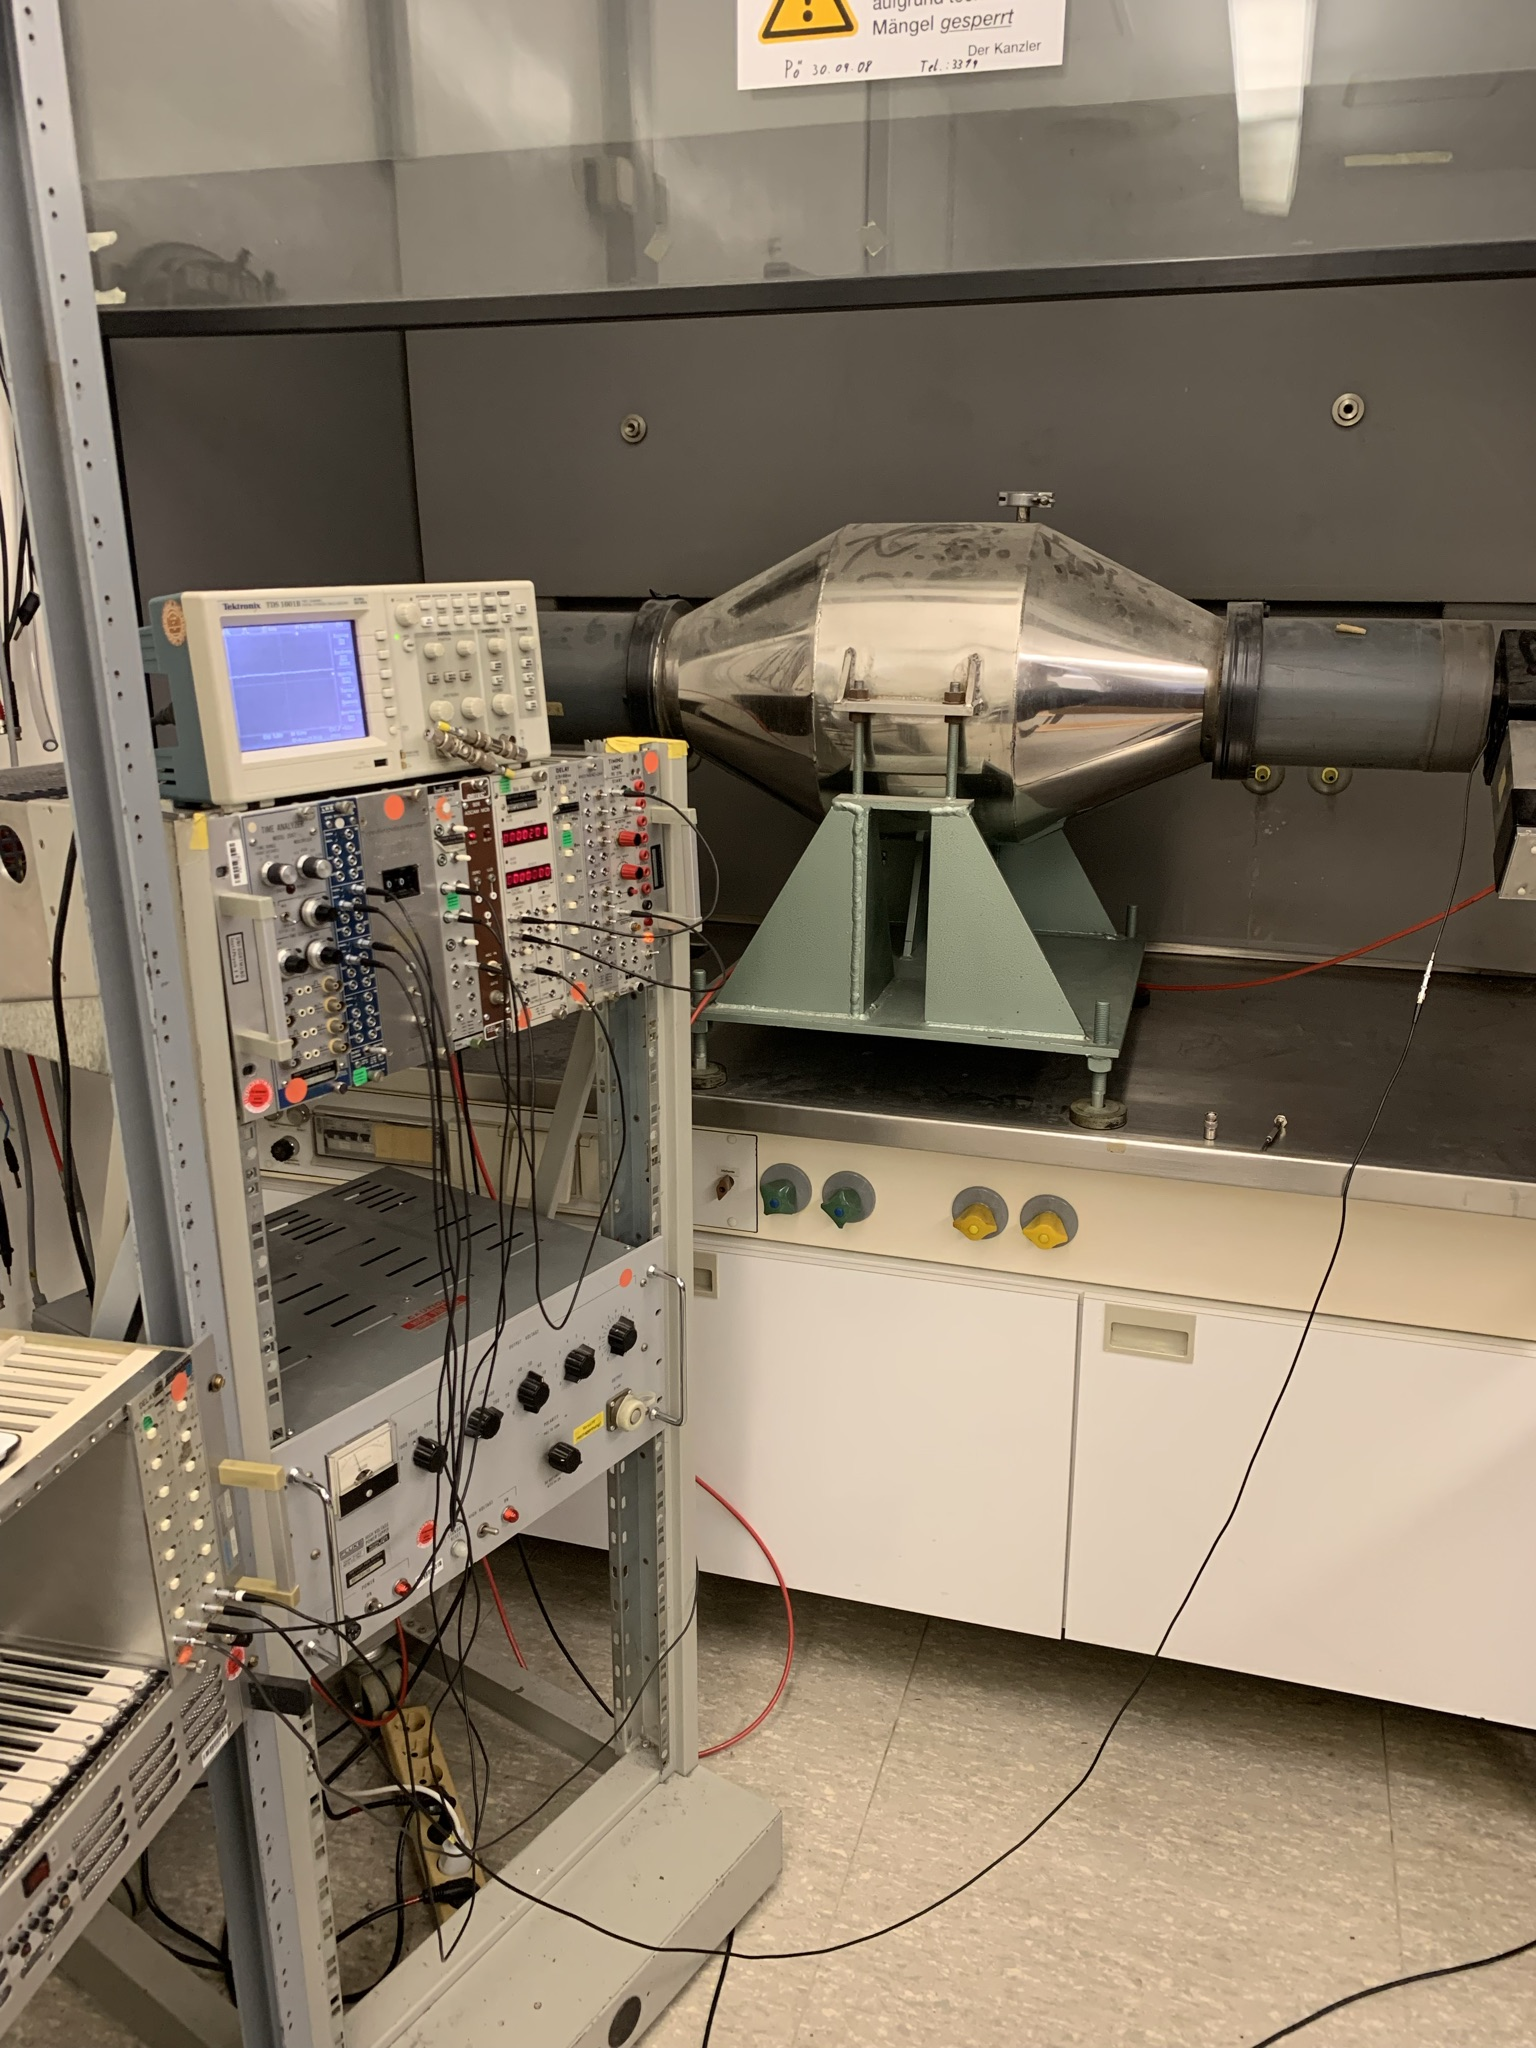
\includegraphics[width=0.8\textwidth]{bilder/bild2.png}
    \caption{hallo}
\end{minipage}
\end{figure}
\vspace{0.5cm}
Die Zeitliche Differenz zwischen den SEVs kann man durch passend eingesetzte \enquote{Delays} entgegenwirken. Diese sind weiter Kabel, 
die durch ihre wählbare Länge die Zeit des Sginals verzögern. So ist es also, dass ein einfallendes Teilchen ein Signal zeitgleich an beiden Anschlüssen ankommen lässt.
Der Aufbau neigt dazu, Störeffekte durch etweige spontane Emission von Elektronen an der Photokathode, zuzulassen. Hier wird ein Diskriminator verwendet, um das Rauschcen zu filtern.
Dieses Bauteil ist direkt mit den SEVs verbunden, es gibt also zwei Individuell einstellbare Diskriminatoren. Bei diesem Elementen ist sowohl
ein \enquote{Threshhold}-, also eine Art Schwelle für die einlaufenden Impulse, und die Breite \enquote{Width} einstellbar.
Die Schwelle ermöglicht es Rauschen aus ungewollten Quellen zu Filtern, mit der Gefahr die Impulse selbst nicht mehr wahrzunehmen. 
Die Breite stellt die elektrische Impulsdauer abhängig von der Einstellung da. Gewählt wurden in dem Versuch $\SI{10}{\nano\second}$ und $\SI{20}{\nano\second}$.
Als zweite Maßnahme wird eine Koinzidenzschaltung dazugeschaltet. In diese Schaltung laufen die wahlweise mehreren Signale, hier zwei, ein und werden nur dann weitergeleited wenn dies gleichzeitig passiert.
Vorzustellen ist dieser Vorgang als logische AND Verknüpfung mit beliebig vielen Bedingungen, die ein Zeitfenster von $\increment t_k$ haben um zu wirken. 
Möglich ist es immer noch für zwei zeitgleich auftretende Emessionen von Elektronen in den SEVs ein fälschliches Signal auszulösen. Die Wahrscheinlichkeit dazu ist aber hinreichend gering
und somit zu vernachläsigen. An dieser Stelle ermöglicht der Aufbau also die hinreichend sichere Detektion von einfallenden Myonen und deren Zerfall, zwischen denm noch nicht unterschieden werden kann. 
\\
\newline
Aussagen über die Lebensdauer von Myonen werden nach \ref{Theorieirgednwoe} durch die Zeit getroffen, die dem Teilchen zwischen dem Einfall in den Szintillator und dem gemessenen 
Zerfall bleibt. Eine Stoppuhr kommt dieser Aufgabe nach, mit der jedoch eine wichtige Bedingung einhergeht. 
Nicht alle Myonen, sogar die wenigsten, zerfallen dort wo ihr Zerfallsimpuls messbar ist. Der Rest geht eben nur mit einem Inititalimpuls einher und verlässt wieder, auf grund zu hoher Energie, den Szintillator.
Es gilt also den Einfall und Zerfall von den Teilchen zu erkennen und messen. Mit der Annahme, der erst gemessene Impuls kommt durch ein einfallendes 
Myon, lässt sich durch den statistischen Fluss an Myonen eine Zeit finden, in der ein weiterer Einfall nahezu unmöglich oder zumindest unwahrscheinlich ist.
In diesem Zeitfenster bietet es sich also an, ungestört nach Zerfallsimpulsen zu suchen. Die Wahl der Suchzeit $\increment T_s$
ist dabei Maßgebend für den Erfolg des Versuchs. Sollte die durchschnittliche Lebensdauer der Myonen überhalb des Zeitfensters liegen, 
bricht die Stoppuhr auch durchschnittlich zu früh die Messung ab und der Zefall wird als Inititalimpuls gewertet. 
Im Aufbau leisten verschiedene Elemente diesen Dienst und liefern so passende Signale die in logischen AND-Gattern entweder die Lebensdauer Messen oder nicht.
Das primäre Signal aus der Koinzidenzschaltung läuft also ungestört in zwei verschiedene AND-Gatter und zusätzlich löst es nach einer Verzögerung von ca $\SI{30}{\nano\second}$
Das Zeitfenster für die Suche aus.
Die zeitliche Abstimmung findet in einem \enquote{Monoflop}, einer Monostabilen Kippstufe, statt. Dieser Monoflop
hat einen Eingang und zwei Ausgänge, wovon einer Invers ist, die für die eingestellte Zeit $\increment T_s$ ein Signal weitergeben. Also sendet ein Ausgang, der mit dem ersten AND-Gatter verbunden ist,
nur bei Aktivierung kein Signal aus. Durch diese Inversität ist gewährleistet, dass nach dem Inititalimpuls kein weiteres Signal die logische und-Bedingung erfüllen kann, bis 
der Monoflop zur Ausgangseinstllung zurückkehrt. Die Verzögerung zum Monoflop erlaubt dem Inititalimpuls die Stoppuhr zu starten. 
Parallel zum ersten AND-Gatter läuft ein zweites Signal vom Monoflop, dieses mal nicht invers, zu einem zweiten AND-Gatter.
Diesem ist also für den Zeitraum $\increment T_s$ ein Signal gegeben und es bedarf nur einem logischen Partner um die und-Bedingung zu erfüllen. 
Das Partnersignal wird hier durch etwaige Impulse im Szintillator gegeben und von der Koinzidenzschaltung direkt zum zweiten AND-Gatter geleitet.
Sollte die Zeit $\increment T_s$ bei einem solchen Event im Monoflop noch nicht agelaufen sein, so ist die und-Bedingung erfüllt,
also das Signal läuft weiter und löst den Stopp für die Zeitmessung aus.
Diese Stoppuhr wird in einem Bauelement namens \enquote{Time to Amplitude Converter} (kurz TAC) realisiert. 
Die hier herausgegene Amplitude ist also proportional zur gemessenen Zeit, die das Myon gebraucht hat um zu zerfallen. Bei erneutem Auslösen des erstem AND-Gatter wird 
im TAC die Zeit neu gestartet.
So ist mit diesem Aufbau möglich Myonen erfolgreich zu detektieren und sogar die, vor dem Zerfall, im Szintillator verbrachte Zeit zu messen.
Um Aufschluss über alle detektierten Teilchen zu bekommen, bietet es sich an gleich hinter dem ersten AND-Gatter zusätzlich einen Impulszähler anzubringen. 
Dieser reagiert auf jedes Signal und erhöht entsprechend den aktuellen Zähler stand. Durch den vorherigen Aufbau lässt es sich so erreichen, dass eben nur die Impulse gezählt werden, die 
in den Szintillator einfallen, keine Zerfälle.
\\
\newline
Zusätzlich gibt es noch einen Doppelimpulsgenerator um wichtige Eigenschaften bei der Auslesung der Amplituden 
richtig einorndnen zu können. Der Generator muss alternativ zum Szintillator an die Koinzidenzschaltung geschlossen werden,
wo er dann zeitlich abgestimmte Impulse gibt. Diese sind einer Skaler am Bauelement zu entnehmen. 
Die weitergeleitete Amplitude wird mit einem System ausgewertet und einem Kanal zugewiesen. Dieser Kanal ist abhängig 
von der Impulsdauer. So lässt sich mit eingigen bekannten Impulsabständen aus dem Generator und dem enstprechend angezeigten Kanälen
feststellen, welcher Kanal bei der echten Messung für welches Zeitintervall $\increment T$ steht.











\begin{figure}
    \centering
    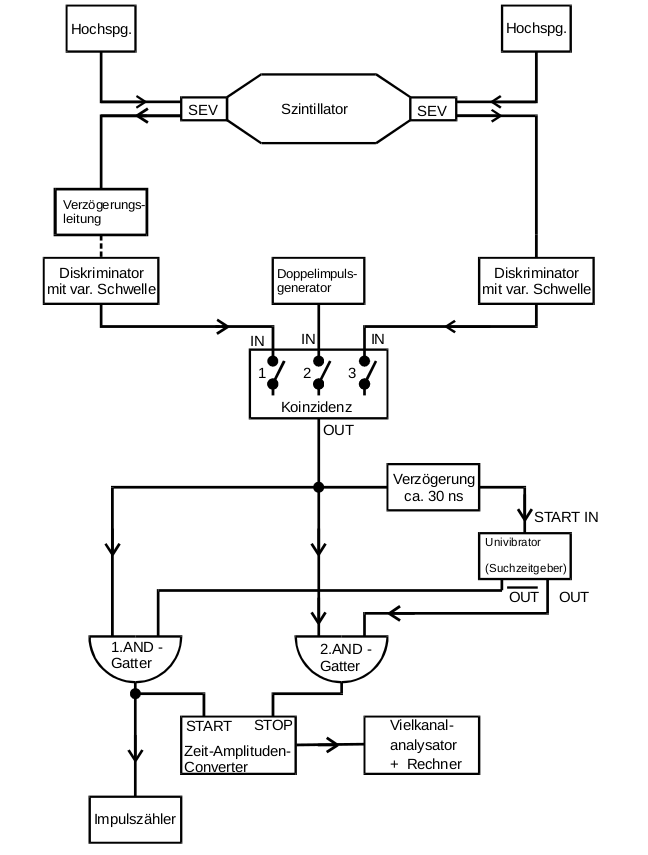
\includegraphics[width=0.9\textwidth]{bilder/aufbau.png}
    \caption{Schematischer Aufbau zur bestimmung der Lebensdauer von Myonen. \cite{skript}} 
    \label{fig:1}
\end{figure}